\documentclass[a4paper,10pt,titlepage]{report}

\usepackage[utf8]{inputenc}
\usepackage{listings}
\usepackage{graphicx}
\usepackage{epstopdf}

%Non sillabare
\tolerance=1
\emergencystretch=\maxdimen
\hyphenpenalty=10000
\hbadness=10000

\lstset{columns=fullflexible,basicstyle=\ttfamily}
\usepackage{graphicx}

\title{MetaC}
\author{TU Delft, Software Engineering Research Group}
\date{Spring 2013}

\begin{document}

\maketitle

\chapter{Introduction}

While the C programming language provides good support for writing efficient, low-level code, it is not adequate for defining higher-level abstractions relevant to embedded software. This project addresses that problem and proposes a language inspired by mbeddr \cite{voelter2012mbeddr} that provides object-oriented functionalities to embedded software developers. 

MetaC results so a domain specific language oriented to the development of reliable and highly maintainable software, equipped with extensions such as State Machine Modelling and Runtime Message Reporting that exempts programmers from writing boilerplate code.

The language has been built on the solid basis of BaseC, that is described in detail in this document, and implemented via Stratego/XT \cite{visser2004program} and Spoofax \cite{kalleberg2007spoofax} technologies. 

Issues as architecture-independence and extensibility have been tackled in the Spring of 2013 at the TU Delft University, during the course of Model-Driven Software Development, by four students leaded by Professor Eelco Visser and supported by the Software Engineering Research Group for one semester.

In the next section, a Conceptual view of mbeddr is given, with references to this project, in order to evidence strengths of both solution. Later, BaseC implementation details are described, with a description of the standard development process used to obtain executable software starting from MetaC programs, and focusing on aspects of syntax and name-binding. 

To follow, the two DSLs for State Machines Modelling and Runtime Message Reporting are described, along with implementation and usage aspects. 

To conclude, a section with future improvements collected during the development of this project takes place. In appendix, a quick reference is provided to be used as handy manual.

\chapter{Conceptual base of mbeddr/MetaC}

mbeddr is a language that provides support for developing embedded software. It enables C programmers to use abstract concepts that are not allowed in standard C as State-Machine-based reasoning or object-oriented modularity. Those concepts can be heavily used for tailoring software to the embedded domain to produce software more maintainable and fixable. Moreover, features that are prohibited in the majority of standards have been removed, in order to keep the software stable and reliable.

The language has been designed with MPS \cite{voelter2010language}, and its approach is radically different from the other embedded development tools in the sense that third parties can use the same mechanisms for building their own extensions that were used to implement C and the existing extensions. 

Also, mbeddr embody tools to support key aspects of the Software Engineering Process as Requirement Verification and Documentation. Via MPS it provides functionalities as such as Model Checking and Contract verification.

MetaC, on the other hand, take only inspiration by mbeddr, and instead of being a projectional language it results as a textual language in order to not need any specific environment to be used in its core functionality. 

It provides support to a big variety of data type that are platform independent, as mbeddr, but also allows old-style C constructs that experienced programmers can exploit to produce very efficient code.

Also, object-oriented reasoning is enabled by the mbeddr-like concept of module and this way C is enriched by features as encapsulation and inheritance that programmers can use in code in an elegant fashion.

State Machines Modelling and Runtime Message Reporting extensions are designed to work also with mbeddr code, so the effort for code migration and maintainability is minimized. Software written using mbeddr can be easily ported to MetaC without apporting too many changes to the source code.


\chapter{BaseC}
\section{Mapping to C and Building}

\begin{figure}[ht!]
\centering
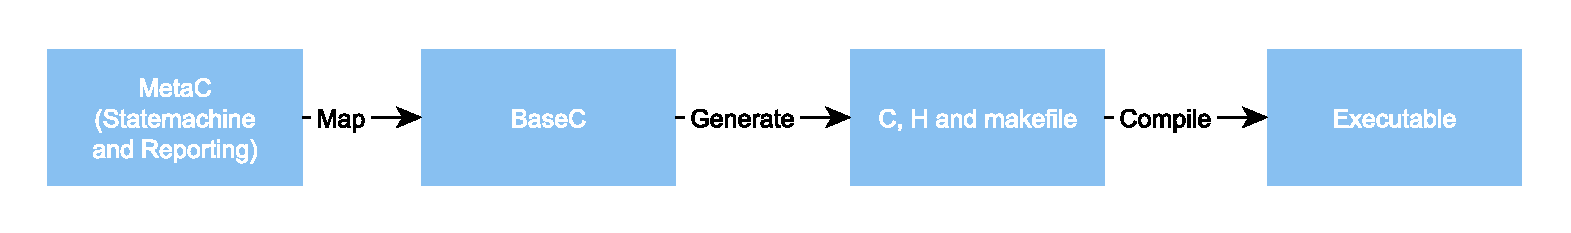
\includegraphics[width=\linewidth]{pics/compilation_simple.eps}
\label{fig:compilation_simple}
\caption{}
\end{figure}

In the bigger picture the mapping from BaseC to C is called the generate step. MetaC is mapped to c and h files together with a make file. Every module generates one c file and one header file. External modules only generate a header file (see next subsection for that). This mapping is based on the way mbeddr maps its modules to c, h and makefile.

The c corresponding to a MetaC module contains:
\begin{itemize}
\item Its corresponding header file
\item The header files of the imported modules
\item Declarations
\item Function definitions
\item Structs, Unions and Enums
\item Components (?)
\item Interfaces (?)
\end{itemize}

The accompanying header file contains:
\begin{itemize}
\item standard ifndef define
\item all external functions
\end{itemize}

The makefile contains:
\begin{itemize}
\item All object file targets for all modules
\end{itemize}
For multiple files the imports are chased recursively. A check is done to ensure modules referenced more than once is only included once in this process. Cyclic references are solved the same way.

\begin{figure}
\centering
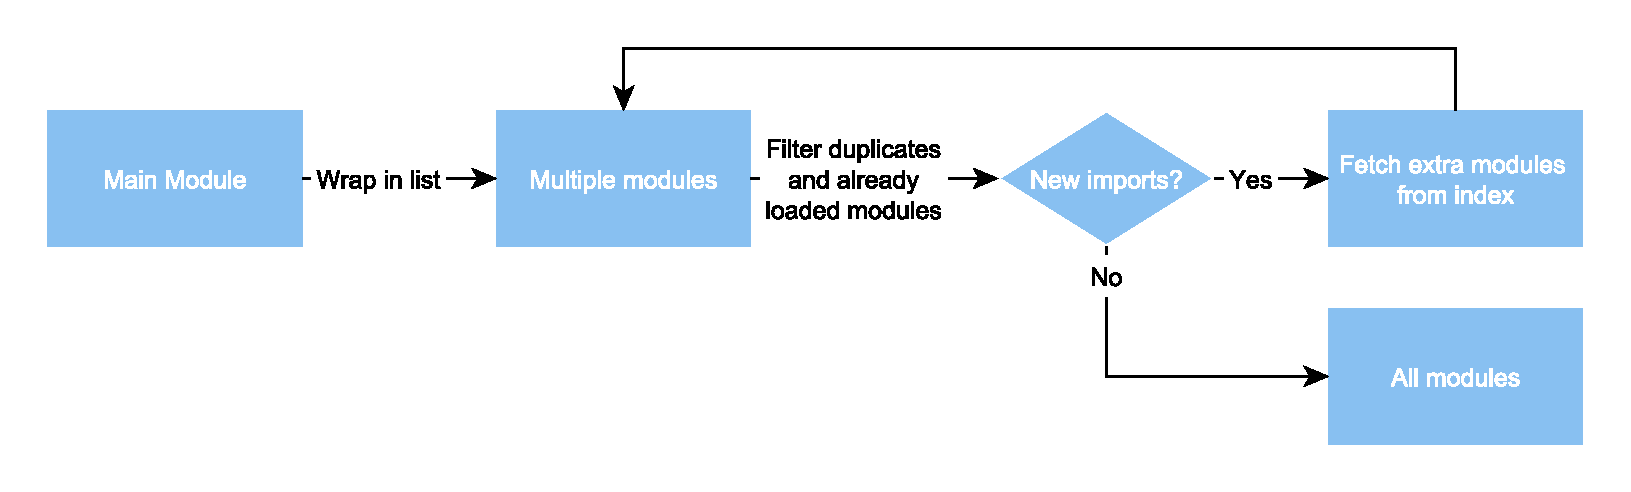
\includegraphics[width=\linewidth]{pics/tracing_imports.eps}
\label{fig:trace_imports}
\caption{Tracing imports}
\end{figure}

After the c files, the headers files and the makefile are generated make with gcc is called, which compiles the program into an executable. As can be seen in the last part of the complete build process.

\begin{figure}[ht!]

\centering
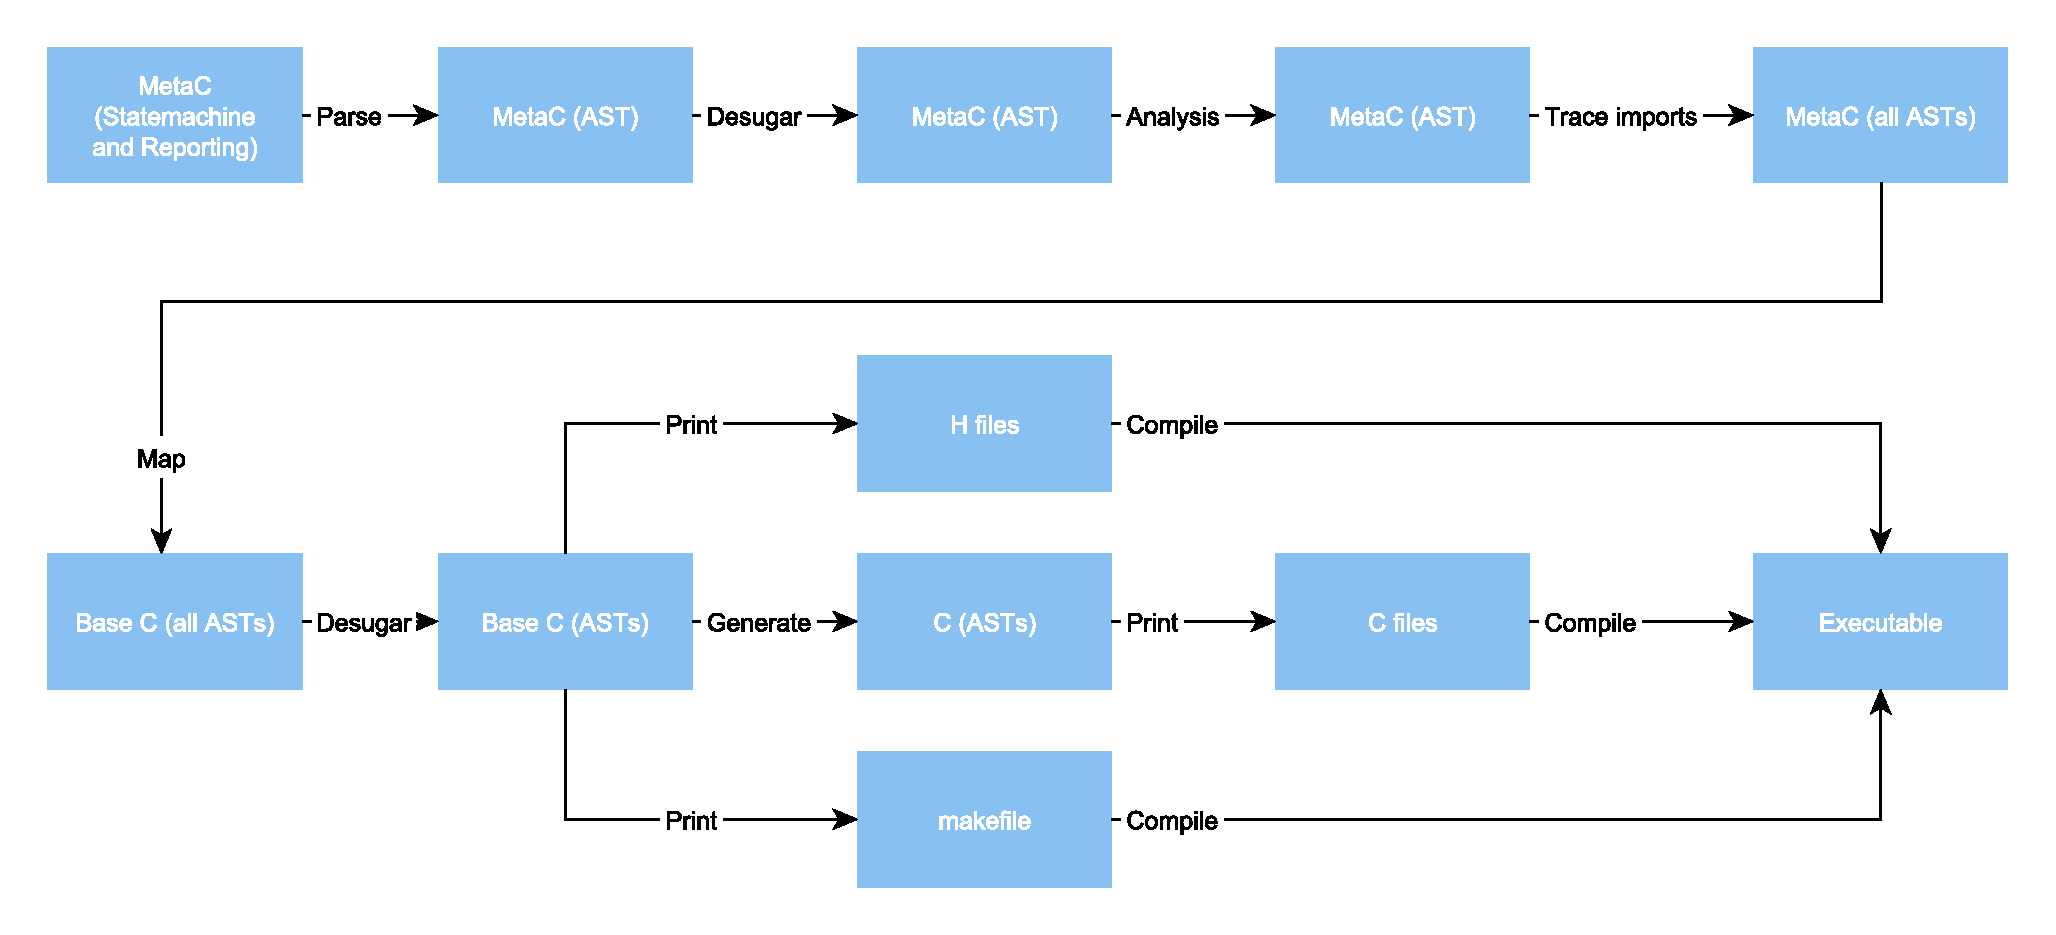
\includegraphics[width=\linewidth]{pics/compilation_complete.eps}
\caption{The complete build process of MetaC}
\label{fig:compilation_complete}
\end{figure}

\subsection{Example program with two modules}
Here we show an example with two modules. The MetaC files (*.mc) show the source code, and the other files the generated c, h and make-file(s) which are fed to gcc.

test52.mc
\begin{lstlisting}
module test52 imports factorial{
       exported int32 main(int32 argc, string[] argv) {
         	printf("5! is %d \n", fact(5));
   	   	return 0;
   	}
}
\end{lstlisting}

factorial.mc
\begin{lstlisting}
module factorial{
   	exported int32 fact(int32 x){
         	if (x <= 1)
                	return 1;
         	return x * fact(x-1);
   	}
}
\end{lstlisting}

test52.h
\begin{lstlisting}
#ifndef TEST52
#define TEST52
 
#include <stdint.h>
 
int32_t main (int32_t argc, int8_t * argv []);
 
#endif
\end{lstlisting}

test52.c
\begin{lstlisting}
#include "test52.h"
#include <stdlib.h>
#include "factorial.h"
int32_t main (int32_t argc, int8_t * argv [])
{
  printf("5! is %d \n", fact(5));
  return(0);
}
\end{lstlisting}

factorial.h
\begin{lstlisting}
#ifndef FACTORIAL
#define FACTORIAL
 
#include <stdint.h>
 
int32_t fact (int32_t x);
 
#endif
\end{lstlisting}

factorial.c
\begin{lstlisting}
#include "factorial.h"
#include <stdlib.h>
int32_t fact (int32_t x)
{
  if((x <= 1))
	return(1);
  return((x * fact((x - 1))));
}
\end{lstlisting}

makefile
\begin{lstlisting}
CC=gcc
CFLAGS=-std=c99
ODIR=./bin
_OBJ_test52=test52.o factorial.o
OBJ_test52=$(patsubst %,$(ODIR)/%,$(_OBJ_test52))
 
 
all: removeStuffFromLibraries clean test52
.PHONY: removeStuffFromLibraries all clean
removeStuffFromLibraries:
   	
$(ODIR)/%.o: %.c
         	mkdir -p $(ODIR)
   	$(CC) $(CFLAGS)   -c -o $@ $< 
debug: CFLAGS +=-g
debug: clean test52
test52: $(OBJ_test52)
   	$(CC) $(CFLAGS) -o $@ $^  
clean:
   	rm -rf $(ODIR) 
\end{lstlisting}

Note that all header files still include <stdint.h> and that all c files still include <stdlib.h> because these are needed for the test programs without external modules. In the future these should be removed.

\chapter{Reporting DSL}
The implementation of the reporting DSL is relatively straightforward. The message constructor has the form 

\emph{Message(id, paramList, modifier, messageText)}

where messageText is a string representing the contents of the message. 

For example: 
\begin{lstlisting}
INFO HelloWorld() inactive: "Hello, World!"
\end{lstlisting}

is parsed to 
\begin{lstlisting}
Message(
  Identifier("HelloWorld"), 
  [], 
  MessageInactive(), 
  String("\"Hello, World!\"")
)
\end{lstlisting}

During indexing, the last term of the constructor (the message text) is stored in the index as \textbf{MsgText()} data. This term (messageText) is later retrieved from the index during the to-basec phase (see the complete build process of MetaC) in order to translate \textbf{Report} statements into \textbf{printf()} function calls. The messageText is used as the parameter for the \textbf{printf()} call.

\chapter{Statemachine DSL}
(intro)
- integration with MetaC
Syntax
[ioana]
-          Definition
-          Calls from BaseC


\chapter{Type checking and name binding}
[ioana]
-          Variables: readable, writable
-          Events (in and out): functions + parameters; condition checking 

\chapter{Mapping to Basec}
[mircea]

\chapter{Future work}
TODO: stuff we didn’t
TODO: brainwaves of stuff we could do
[everybody]

MetaC is a solid base for future expansions. The language provides basic functionality with modules and has the reporting and statemachine DSLs. Suggested features for future work can be found on the issue tracker of MetaC.
\section{Import all std. C libraries automatically}
One suggestion to improve MetaC is to automatically generate all external modules wrapping C standard libraries. The glibc is however full of macros, which make it non trivial to extract the external function definitions. Discussing this feature can be done on the issue tracker.
\section{Import custom C libraries}
An important feature for MetaC is the use of external custom C libraries. This is important as developers can keep using existing systems and build MetaC on top of these systems. As with the standard C libraries this could be done automatically too. Based on the amount of macros in these custom libraries this might either be easy or not. Writing a generic solution would mean ignoring macros, since tracing al macro logic is nearly impossible.
\section{Variable argument function definitions}
In order to support variable argument functions for standard C libraries these variable argument functions need to be supported in MetaC themselves. Since functions like printf are often used this would be a very appreciated improvement. For developers of embedded software this might be less important since embedded programming is usually conservative in use of features for performance and reliability.

\bibliographystyle{plain}
\bibliography{metac}

\appendix
\chapter{Appendix A: quick reference}
\section{Datatypes}
In table X is reported a list of data types implemented in the syntax of MetaC, with reference to the equivalent standard C data type and size of the type

\begin{tabular}{|l|l|l|}
\hline
MetaC & Standard C & Size [bit] \\ \hline
boolean & - & -\\ 
int8 & char & 8 \\ 
int16 & short & 16 \\ 
int32 & int & 32 \\ 
int64 & long long & 64 \\ 
uint8 & unsigned char & 8 \\ 
uint16 & unsigned short & 16 \\ 
uint32 & unsigned int & 32 \\ 
uint64 & unsigned long long & 64 \\ 
float & float & 32 \\ 
double & double & 64 \\ 
string & - & - \\
\hline
\end{tabular}


\section{Modules}
The top level concept in MetaC programs are modules. Modules act as namespaces and as the unit of encapsulation. The classical separation between .c and .h files doesn’t exists in MetaC, the code takes place in .mc files that get transformed to .c and .h files during the generation phase. 
A module can import other modules. The importing module can then access the exported contents of imported modules. Module contents can be exported using the keyword exported.

A basic module is shown in code snippet X.

\begin{lstlisting}
module HelloWorld imports nothing {
    int32 main() {
		return 0;
	}
}
\end{lstlisting}

\section{Limitations on pointer arithmetic}
Pointer arithmetics 
\section{non decimal numbers}
[dario]


\end{document}
